\chapter{Lindenmayer-Systeme}

Vorstellung der verwendeten Konzepte. Sämtliche Visualisierungen von L-Systemen wurden mithilfe des Unreal Engine 4 Projekts erstellt.

\section{Kontextfreie Grammatik}

Bei L-Systemen handelt es sich um, auf Zeichenketten basierende, Ersetzungssysteme. Es werden komplexe Objekte beschrieben, indem Teile der Zeichenkette durch andere Zeichen oder Zeichenketten ersetzt werden. Die Beschreibung dieser Ersetzungen findet mittels festgelegter Produktionsregeln statt. \cite[S.2]{ABOP:04} 

Eine formale Definition eines auf Zeichenketten arbeitenden Ersetzungssystems wird durch kontextfreie Grammatiken gegeben:

\newtheorem{defKontextfreieGrammatik}{Kontextfreie Grammatik:}[chapter]
\begin{defKontextfreieGrammatik}
	Eine kontextfreie Grammatik G ist ein Tupel G = $(V, N, P, \omega)$ bestehend aus:
	\begin{enumerate}
		\item $V$ -- einer nichtleeren, endlichen Menge von Buchstaben (Alphabet).
		\item $N$ -- einer endlichen Menge von Variablen.
		\item $P$ -- einer endlichen Menge von Produktionsregeln in der Form $P: A \rightarrow \alpha$ mit $A \in N$ und $\alpha \in (V \cup N )^*$.
		\item $\omega \in N$ -- dem Axiom, Startsymbol der Grammatik.
	\end{enumerate}
	\cite[S.343]{ThI:14}
\end{defKontextfreieGrammatik}

Die Menge $V^*$ ist die Menge aller Wörter über $V$ -- die Menge aller Wörter, die aus dem Alphabet $V$ gebildet werden können. \cite[S.70]{ThI:14} 

Eine Grammatik wird als kontextfrei bezeichnet, wenn beispielsweise die Produktionsregel $A \rightarrow \alpha$ angewendet werden kann, ohne die $A$ umgebenden Buchstaben -- seinen Kontext -- beachten zu müssen. \cite[S.343]{ThI:14} 

Eine Grammatik wird als deterministisch bezeichnet, wenn es genau eine Produktionsregel $r \in P$ für jede Variable $A \in V$ gibt, sodass $r: A \rightarrow \alpha$, $\alpha \in (V \cup N )^*$. Das bedeutet, dass die Ersetzung einer Variable eindeutig durch eine einzige Regel beschrieben wird. \cite[S.75]{PCGiG:16}

Die Anwendung der Produktionsregeln findet meist sequentiell statt -- die Zeichenkette wird von links nach rechts durchlaufen und Ersetzungen werden direkt auf die untersuchte Zeichenkette angewendet. \cite[S.75]{PCGiG:16}

\section{D0L-Systeme}

Diese Arbeit beschränkt sich auf die Behandlung deterministischer, kontextfreier L-Systeme, auch D0L-Systeme genannt. Diese besitzen die Eigenschaften einer deterministischen und kontextfreien Grammatik, Produktionsregeln werden jedoch parallel und gleichzeitig auf alle Buchstaben des untersuchten Wortes angewendet. Dieses Vorgehen soll die Zellteilung in mehrzelligen Organismen simulieren und ist somit an biologische Vorgänge angelehnt. \cite[S. 3]{ABOP:04} 

Ein D0L-System kann wie folgt definiert werden:
\newtheorem{defD0LSystem}{D0L-System:}[chapter]
\begin{defD0LSystem}
	Ein D0L-System ist ein Tupel G = $(V, P, \omega)$, bestehend aus
	\begin{enumerate}
		\item $V$ -- einem nichtleeren, endlichen Alphabet.
		\item $P$ -- einer endlichen Menge von Produktionsregeln in der Form $P: a \rightarrow b$ mit $a \in V$ und $b \in V^*$. $a$ wird als Vorgänger, $b$ als Nachfolger bezeichnet. Ist für einen Buchstaben $x \in V$ keine explizite Produktionsregel angegeben, wird die Identitätsproduktion $P: x \rightarrow x$ angenommen -- der Buchstabe wird durch sich selbst ersetzt.
		\item $\omega \in V^+$ -- dem Axiom, Startsymbol der Grammatik.
	\end{enumerate}
Die Menge $V^+$ ist die Menge aller nichtleeren Wörter über $V$. \cite[S.4]{ABOP:04} 
\end{defD0LSystem}

Die Ableitung eines Wortes entspricht der Ersetzung aller Buchstaben anhand der Produktionsregeln. Ein Wort kann mehrmals abgeleitet werden. 

\newtheorem{defAbleitung}{Ableitung:}[chapter]
\begin{defAbleitung}
	Gegeben sei ein Wort $w = a_1 ... a_m$ mit $w \in V^*$ und $a_i \in V^*$. Das Wort $v = b_1 ... b_m$ mit $v \in V^*$ und $b_i \in V^*$ ist die Ableitung von $w$ wenn für alle $i=1...m$ eine Produktionsregel $a_i \rightarrow b_i$ existiert. Die Ableitung wird als $w \Rightarrow v$ notiert. \\
	Das Wort $w_n$ ist die n-te Ableitung des Wortes $w_0$ wenn eine Folge von Wörtern $w_0, w_1, ..., w_n$ mit Ableitungen $w_0 \Rightarrow w_1 \Rightarrow ... \Rightarrow w_n$ existiert. \cite[S.4]{ABOP:04} 
\end{defAbleitung}


Beispiel: Das Wachstum der Blaualgen-Gattung \glqq Anabaena\grqq{} kann durch ein L-System simuliert werden. Die Buchstaben $a$ und $b$ beschreiben die Größe und Teilungsbereitschaft einer Algenzelle, während die Indizes $l$ und $r$ die Polarität einer Zelle darstellen. Es gelten folgende Produktionsregeln:
\begin{equation}
\begin{array}{cccc}
 p_1 & : a_r &\rightarrow& a_lb_r \\
p_2 &  : a_l &\rightarrow& b_la_r \\ 
p_3 &  : b_r &\rightarrow& a_r \\
p_4 &  : b_l &\rightarrow& a_l 
\end{array}
\label{eq:ProdAnabaena}
\end{equation} 

Die Entwicklung einer Anfangszelle $a_r$ (Axiom $\omega : a_r$) läuft daraufhin wie in Abbildung \ref{fig:AnabaenaAbleitung} dargestellt ab.
\begin{figure} [hbtp]
	\centering
	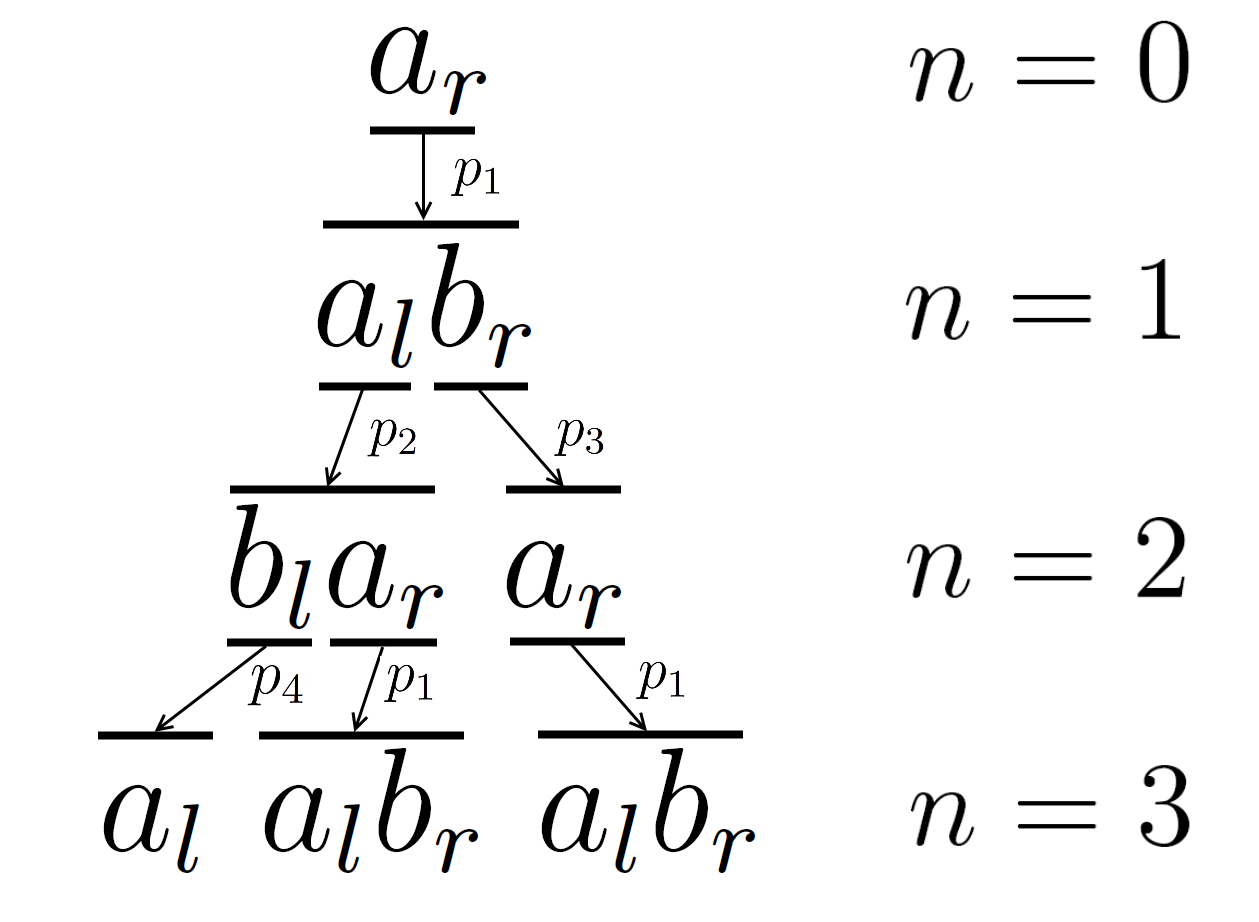
\includegraphics[height=0.3\textheight]{images/AnabaenaAbleitung.png}
	\caption{n-fache Ableitung der Anfangszelle $a_r$ anhand der Produktionsregeln $p_1 ... p_4$ aus Gleichung \ref{eq:ProdAnabaena}. Eigene Abbildung anhand \cite[S.4]{ABOP:04}}
	\label{fig:AnabaenaAbleitung}
\end{figure}

\subsection{Parametrische L-Systeme}

Parametrische L-Systeme stellen eine Erweiterung der D0L-Systeme dar. Die Buchstaben eines verwendeten Alphabets $V$ werden um zugeordnete Parameter aus der Menge der reelen Zahlen ergänzt. Ein solches parametrisches Wort $V \times \Re^*$ besteht aus einem Zeichen $A \in V$ und Parametern $a_1,...,a_n \in \Re$ und wird als $A(a_1,...,a_n)$ dargestellt. Ein parametrisches Wort ohne Parameter mit dem Zeichen $A \in V$  wird schlicht als $A$ dargestellt. \cite[S.41]{ABOP:04}

Während in der Definition von Modulen numerische Konstanten verwendet werden, werden bei der Angabe eines L-Systems Variablen verwendet. Ist $\Sigma$ eine Menge von Variablen, dann ist $E(\Sigma)$ ein arithmetischer Ausdruck, in dem Variablen, Konstanten und arithmetische Operatoren auf eine zulässige Weise kombiniert werden. \cite[S.41]{ABOP:04}

\newtheorem{defParametrischeLSysteme}{Parametrisches L-System:}[section]
\begin{defParametrischeLSysteme}
	Ein Parametrisches L-System ist ein Tupel G = $(V, \Sigma, P, \omega)$, bestehend aus
	\begin{enumerate}
		\item $V$ -- einem nichtleeren, endlichen Alphabet.
		\item $\Sigma$ -- einer Menge der Variablen.
		\item $P$ -- einer endlichen Menge von Produktionsregeln $P : (V\times \Sigma^*) \rightarrow (V\times E(\Sigma))^*$
		\item $\omega \in M^+$ mit $M =(V \times \Re^*)$ -- einem Axiom in Form eines nichtleeren, parametrischen Wortes.
	\end{enumerate}
\cite[S.41]{ABOP:04}
\end{defParametrischeLSysteme}

Eine Produktion kann auf ein parametrisches Wort angewendet werden wenn das Zeichen, das dem Wort vorausgeht, und die Anzahl der Parameter mit dem Zeichen und der Anzahl der Parameter im Vorgänger der Produktionsregel übereinstimmen. \cite[S.42]{ABOP:04}

Beispiel: Gegeben sei folgendes, parametrisches L-System:

\begin{equation}
\begin{array}{llll}
\omega & : A(1,1) \\
p_1 & : A(x,y) &\rightarrow& A(x+1, y*2)\text{ }B(y) \\
p_2 &  : B(x) &\rightarrow& B(x+1)\text{ }C 
\end{array}
\label{eq:ProdParamLSystem}
\end{equation} 

Das Alphabet $V$ und die Menge der Variablen $\Sigma$ gehen implizit aus der Angabe der Produktionsregeln hervor und werden in zukünftigen L-System-Gleichungen nicht angegeben. Die Entwicklung des L-Systems läuft anhand Abbildung \ref{fig:ParamLSystemBeispiel} ab. 

\begin{figure} [hbtp]
	\centering
	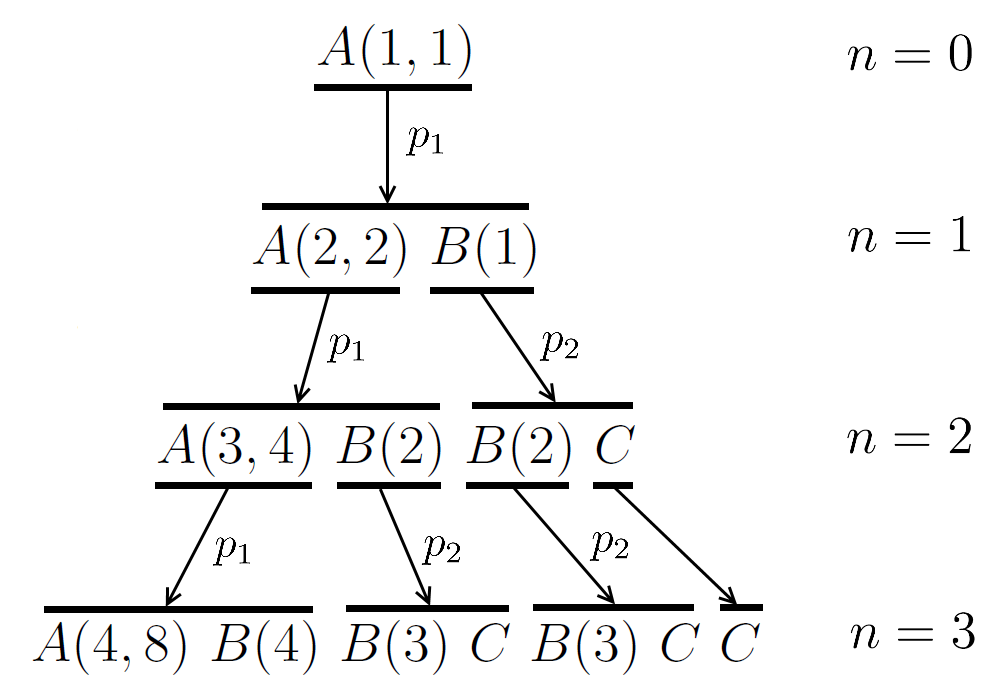
\includegraphics[height=0.4\textheight]{images/ParamLSystemBeispiel.png}
	\caption{n-fache Ableitung des Axioms $A(1,1)$ anhand der Produktionsregeln aus Gleichung \ref{eq:ProdParamLSystem}. Die Ersetzung des Zeichens $C$ erfolgt anhand der impliziten Identitätsproduktion. Eigene Abbildung.}
	\label{fig:ParamLSystemBeispiel}
\end{figure}

\section{Grafische Interpretation von L-Systemen}

Um die Ergebnisse von L-Systemen in Form von dreidimensionalen Objekten zu visualisieren, muss eine grafische Interpretation der resultierenden Zeichenketten festgelegt werden. Im Folgenden wird die verwendete Visualisierungsmethode, Turtle-Interpretation, vorgestellt.

\subsection{Turtle-Interpretation}

Die Turtle-Interpretation im zweidimensionalen Raum entspricht der Vorstellung einer Turtle\footnote{\glqq Turtle\grqq{} -- englisch für \glqq Schildkröte\grqq.} auf einem Blatt Papier. Die Turtle besitzt eine Position $\overrightarrow{P}$ welche durch die kartesischen Koordinaten $(p_1,p_2)$ beschrieben wird sowie einen Einheitsvektor $\overrightarrow{H}$ mit kartesischen Koordinaten $(h_1, h_2)$. $\overrightarrow{P}$ beschreibt die Position der Turtle auf der Ebene und $\overrightarrow{H}$ entspricht der Blickrichtung (Heading) der Turtle. Der Zustand $(\overrightarrow{P},\overrightarrow{H})$ einer Turtle wird somit vollständig durch die Position und Blickrichtung definiert. \cite[S.2]{Turtle:04} Die Turtle kann drei Aktionen durchführen, welche durch die folgenden Symbole dargestellt werden:

\begin{description}[labelindent]
	\item[$F(a)$] Die Turtle bewegt sich um $a>0$ in die Richtung der aktuellen Blickrichtung. Die neue Position ist  $\overrightarrow{P'} = (p_1',p_2')$ mit:
	\begin{equation}
	\begin{array}{ll}
	p_1' & = p_1 + h_1 * a\\
	p_2' & = p_2 + h_2 * a
	\end{array}
	\end{equation} 
	Zwischen der alten Position $\overrightarrow{P}$ und der neuen Position $\overrightarrow{P'}$ wird eine Linie gezeichnet.
	
	\item[$+(a)$]  Die Turtle dreht sich um den Winkel $a$ nach links. Die neue Blickrichtung ist $\overrightarrow{H'} = (h_1', h_2')$ mit:
	\begin{equation}
	(h_1', h_2') = (h_1, h_2) *
	\begin{pmatrix}
	cos(a) & sin(a)\\
	-sin(a) & cos(a)
	\end{pmatrix}
	\end{equation} 
	
	\item[$-(a)$]  Die Turtle dreht sich um den Winkel $a$ nach rechts. Die neue Blickrichtung ist $\overrightarrow{H'} = (h_1', h_2')$ mit:
	\begin{equation}
	(h_1', h_2') = (h_1, h_2) *
	\begin{pmatrix}
	cos(-a) & sin(-a)\\
	-sin(-a) & cos(-a)
	\end{pmatrix}
	\end{equation} 
	
\end{description}
\cite[S.4,46]{Turtle:04} \cite[S.7]{ABOP:04}
Die Symbole \glqq+\grqq{} und \glqq-\grqq{} werden sowohl im Alphabet eines L-Systems als auch bei arithmetischen Operationen in Parameterangaben verwendet, ihre Bedeutung ist abhängig vom Kontext, in welchem sie angewendet werden. \cite[S.46]{ABOP:04}

Die grafische Turtle-Interpretation einer Zeichenkette, die durch ein L-System zurückgegeben wird, sind somit die Linien, die auf Grundlage der definierten Symbole gezeichnet werden. 

Beispiel: Mithilfe von L-Systemen und einer Turtle-Interpretation können Fraktale, in diesem Beispiel sogenannte Koch-Kurven visualisiert werden. Diese Kurven bestehen aus einem Initiator -- einer einfachen, zweidimensionalen Form -- und einem Generator, der einem offenen Polygonzug entspricht. In jedem Ableitungsschritt, angefangen bei dem Initiator, wird jede gerade Linie durch den Generator ersetzt. \cite[S.39]{Mandelbrot:16} 

Dieses Verhalten kann nun auf ein L-System abgebildet werden: Der Initiator entspricht dem Axiom und der Generator einer Produktionsregel des L-Systems. Der in Abbildung \ref{fig:InitiatorGenerator} dargestellte Initiator und Generator entsprechen der Turtle-Interpretation des folgenden L-Systems:

\begin{figure} [hbtp]
	\centering
	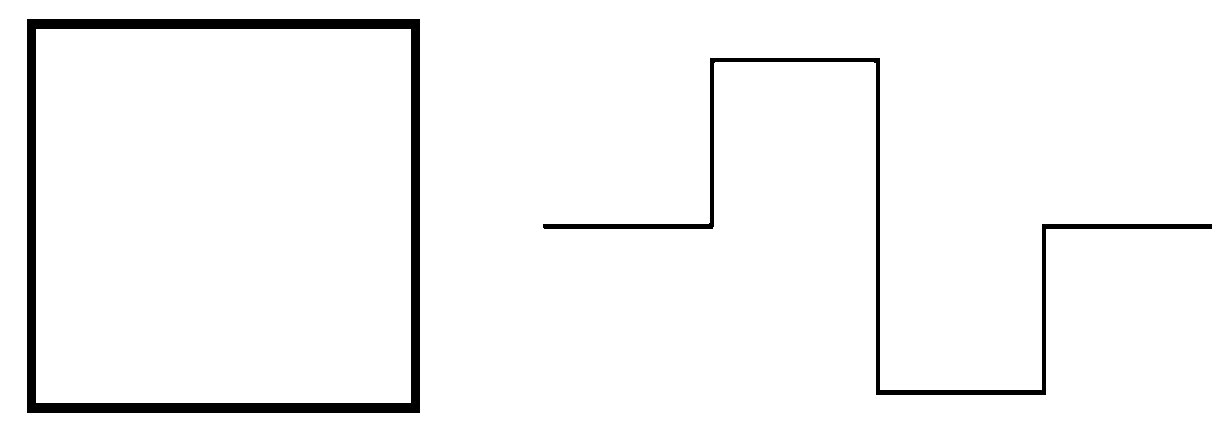
\includegraphics[width=0.6\textwidth]{images/InitiatorGenerator.png}
	\caption{Links: Initiator der Koch-Kurve in Form eines einfachen Quadrats. Rechts: Generator der Koch-Kurve in Form eines offenen Polygonzugs. Eigene Abbildung.}
	\label{fig:InitiatorGenerator}
\end{figure}

\begin{equation}
\begin{array}{llll}
\omega & : F-F-F-F \\
p_1 & : F \rightarrow F+F-F-FF+F+F-F
\end{array}
\label{eq:ProdKochKurve}
\end{equation} 

Für eine bessere Übersicht wurde die Angabe der Parameter weggelassen. Die Turtle interpretiert $F$ als $F(l)$, $-$ als $-(d)$ und $+$ als $+(d)$ mit festgelegter Strichlänge $l$ und Drehwinkel $d$. \label{desc:TurtleWithoutParams} Die Entwicklung des L-Systems läuft, als Turtle-Interpretation visualisiert, wie in Abbildung \ref{fig:KochkurveAbleitung} ab.

\begin{figure} [hbtp]
	\centering
	\begin{subfigure}[t]{.3\textwidth}
		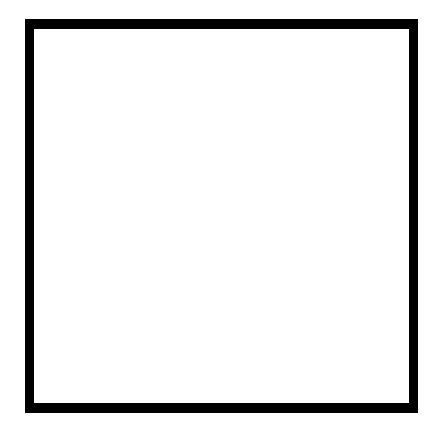
\includegraphics[width=\linewidth]{images/KochkurveN0L400.png}
		\caption{$n=0$, $l=400$, $d=90\degree$}
		\label{fig:KochkurveN0L400}
	\end{subfigure}
	\hspace{.1\textwidth}
	\begin{subfigure}[t]{.3\textwidth}
		\centering
		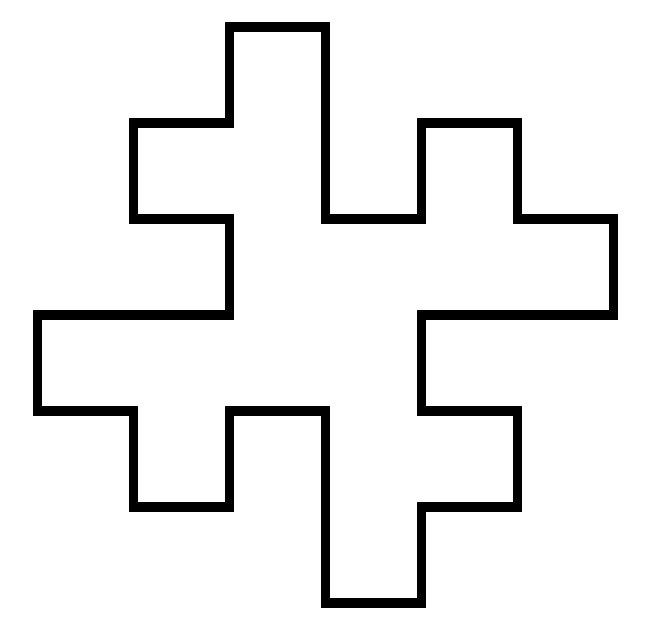
\includegraphics[width=\linewidth]{images/KochkurveN1L100.png}
		\caption{$n=1$, $l=100$, $d=90\degree$}
		\label{fig:KochkurveN1L100}
	\end{subfigure}
	\medskip
	\begin{subfigure}[t]{.3\textwidth}
		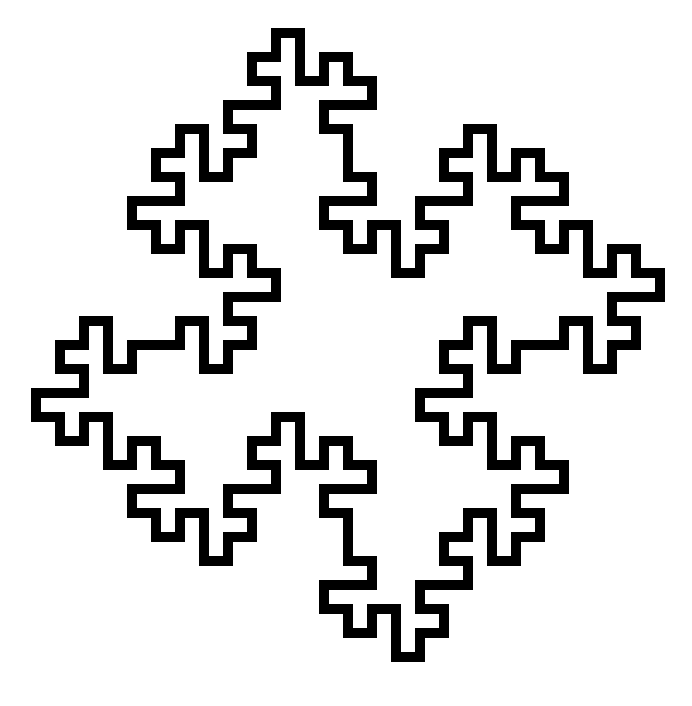
\includegraphics[width=\linewidth]{images/KochkurveN2L25.png}
		\caption{$n=2$, $l=25$, $d=90\degree$}
		\label{fig:KochkurveN2L25}
	\end{subfigure}
	\hspace{.1\textwidth}
	\begin{subfigure}[t]{.3\textwidth}
		\centering
		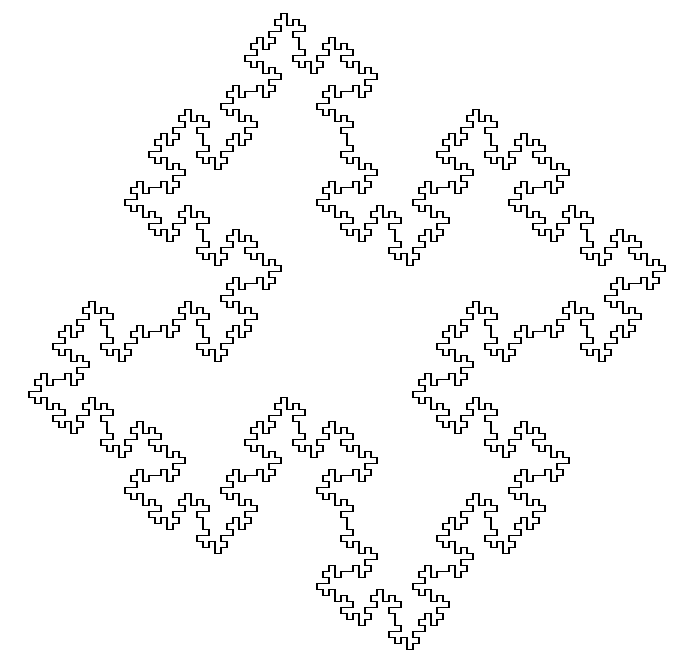
\includegraphics[width=\linewidth]{images/KochkurveN3L6_25.png}
		\caption{$n=3$, $l=6.25$, $d=90\degree$}
		\label{fig:KochkurveN3L6_25}
	\end{subfigure}
	\caption{n-fache Ableitung des Axioms $\omega$ anhand der Produktionsregel $p_1$ aus Gleichung \ref{eq:ProdKochKurve}, visualisiert mithilfe der Turtle-Interpretation. Die im Parameter $l$ verwendete Einheit entspricht der in der Unreal Engine 4 verwendeten Längeneinheit $cm$. Eigene Abbildung.}
	\label{fig:KochkurveAbleitung}
\end{figure}

\subsection{Verzweigte L-Systeme}

Die bisherigen Definitionen von L-Systemen und die korrespondierende Turtle-Interpretation lässt lediglich die Bildung von Grafiken zu, die einen einzelnen, zusammenhängenden Polygonzug erlauben. Um L-Systeme zu bilden, deren Visualisierungen Baumstrukturen ähneln muss die bisherige Turtle-Interpretation um die Möglichkeit erweitert werden, Verzweigungen zu verarbeiten. \cite[S.24]{ABOP:04} 

Folgende Operationen werden eingeführt:

\begin{description}[labelindent]
	\item[$\text{[}$] Der aktuelle Zustand der Turtle in Form ihrer Position und Rotation wird auf einem Kellerspeicher abgelegt. \\
	
	\item[$ \text{]} $] Der oberste Zustand der Turtle wird vom Kellerspeicher genommen. Die aktuelle Position und Rotation der Turtle wird auf die im Zustand gespeicherte Position und Rotation gesetzt. Es wird keine Linie zwischen der alten und neuen Position gezeichnet.
\end{description}
	\cite[S.24]{ABOP:04} 

Diese Erweiterung erlaubt es mehrere Linien zu zeichnen, die von einem einzigen Punkt ausgehen -- die Visualisierung von Abzweigungen ist somit möglich. Die Operatoren [ und ] markieren den Anfang und das Ende eines Zweiges.

Beispiel: Mithilfe von verzweigten L-System-Beschreibungen lassen sich simple, Baum- oder Strauch-ähnliche Strukturen bilden. Die Turtle-Interpretation folgt der in \ref{desc:TurtleWithoutParams} beschriebenen Interpretation mit fester Strichlänge $l$ und festem Drehwinkel $d$.


\begin{figure} [hbtp]
	\centering
	\begin{subfigure}[t]{.4\textwidth}
		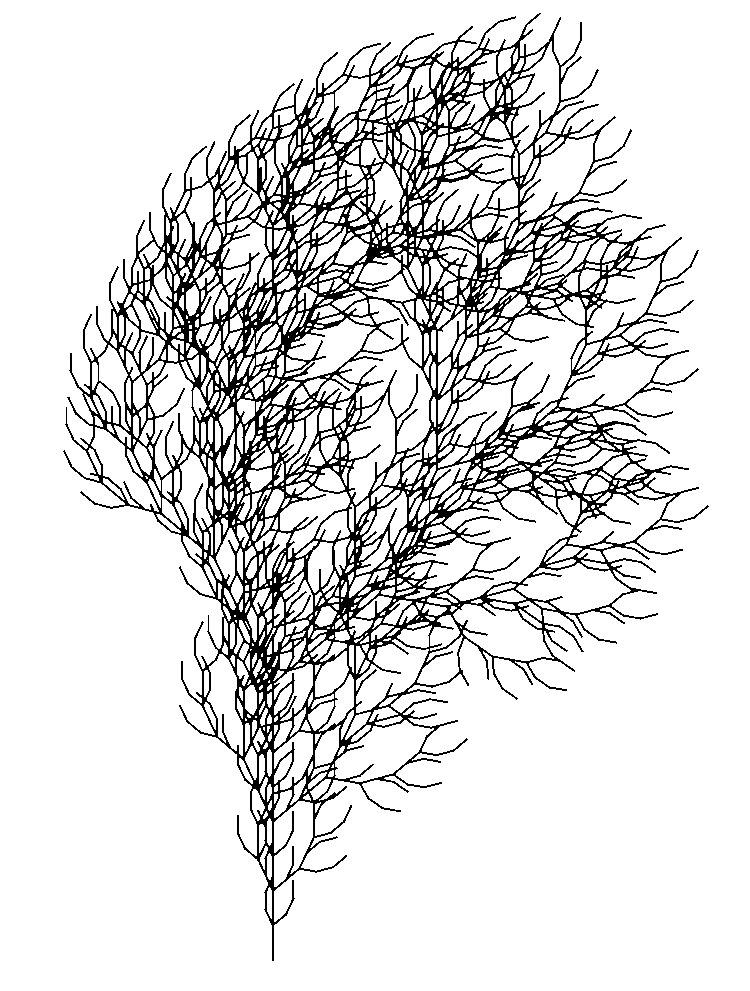
\includegraphics[width=\linewidth]{images/Branching1_N4L18D25.png}
		\caption{$n=4$, $l=18$, $d=25\degree$\\ \\
			$\begin{array}{ll}
				\omega & : F \\
				p_1 & : F \rightarrow FF-[-F+F+F]+[+F-F-F]
			\end{array}
			\label{eq:ProdBranching1}$\\
			\cite[S.25]{ABOP:04}
		}
		\label{fig:Branching1L18D25}
	\end{subfigure}
	\hspace{.1\textwidth}
	\begin{subfigure}[t]{.4\textwidth}
		\centering
		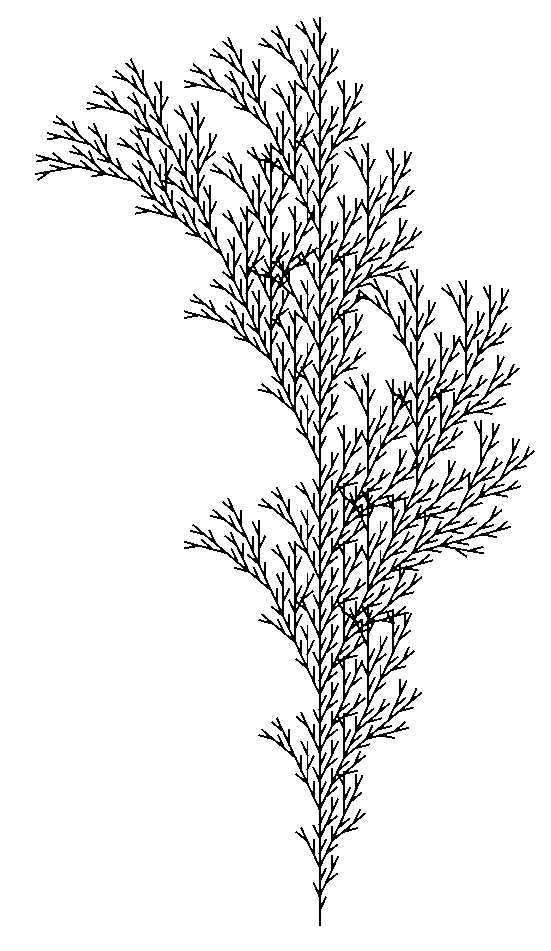
\includegraphics[width=\linewidth]{images/Branching2_N5L15D25.png}
		\caption{$n=5$, $l=15$, $d=25\degree$\\ \\
			$\begin{array}{ll}
				\omega & : F \\
				p_1 & : F \rightarrow F[-F]F[+F][F]
			\end{array}
			\label{eq:ProdBranching2}$\\
			\cite[S.78]{PCGiG:16}
		}
		\label{fig:Branching2L15D25}
	\end{subfigure}

	\caption{n-fache Ableitung der Axiome anhand der Produktionsregeln, visualisiert mithilfe der Turtle-Interpretation. Eigene Abbildung.}
	\label{fig:KochkurveAbleitung}
\end{figure}

\subsection{Erweiterung der Turtle-Interpretation in den dreidimensionalen Raum}

Die bisherige Definition eines Turtle-Zustands mithilfe einer zweidimensionalen Position und einer Blickrichtung genügt nicht, um Visualisierungen von L-Systemen in Form von dreidimensionalen Objekten zu ermöglichen. Sowohl die Zustands-Definition als auch die interpretierten Operationen müssen angepasst und erweitert werden.

Der Zustand der Turtle im dreidimensionalen Raum besitzt eine Position $\overrightarrow{P}$ sowie drei Einheitsvektoren $\overrightarrow{H}$, $\overrightarrow{U}$ und $\overrightarrow{L}$, welche die Orientierung der Turtle im Raum in kartesischen Koordinaten beschreiben. Die Orientierungsvektoren sind orthogonal zueinander und bilden somit das lokale Koordinatensystem der Turtle.

\begin{description}[5cm]
		\item[\boldmath$\overrightarrow{H}$]Entspricht der Blickrichtung (Heading) der Turtle. Eine Rotation um diesen Vektor entspricht der Rotationsmatrix \\
		\begin{equation}
		\begin{pmatrix}
		cos(d) & sin(d) & 0 \\
		-sin(d)& cos(d) & 0 \\
		0 & 0 & 1
		\end{pmatrix}	
		\label{eq:rotH}
		\end{equation} 
		\item[\boldmath$\overrightarrow{U}$]Entspricht dem Vektor, der im lokalen Koordinatensystem der Turtle nach oben zeigt (Up).\\
		\begin{equation}
		\begin{pmatrix}
		cos(d) & sin(d) & 0 \\
		-sin(d)& cos(d) & 0 \\
		0 & 0 & 1
		\end{pmatrix}	
		\label{eq:rotU}
		\end{equation} 
		\item[\boldmath$\overrightarrow{L}$]Entspricht dem Vektor, der im lokalen Koordinatensystem der Turtle nach links zeigt (Left).
\end{description}

\cite[S.19]{ABOP:04}



\begin{description}[5cm]
	\item[\boldmath$+(d)$ und $-(d)$]  Die Turtle dreht sich um den \\
	
	\item[\boldmath$/(d)$ und $\backslash(d)$]test \\
	
	\item[\boldmath
	$
	\begin{array}{cc}
	+(d)\\-(d)
	\end{array}
	$] Entspricht dem Vektor, der im lokalen Koordinatensystem der Turtle nach links zeigt (Left).
\end{description}
